\chapter{Cylindrical Simulations to Study the Effect of Beam Radius in Direct-Drive}

This chapter describes a cylindrical, direct-drive implosion simulation platform and corresponding ensemble of simulations that was developed to study the effect of the beam radius initial condition on \textsc{Omega} laser facility experiments.
Although results from the cylindrical simulations do not have the same convergence properties of spherical implosions, much of the essential physics which is important to studying the effect of beam radius is preserved.
The main benefit of the geometry is that a 2-D ray-trace can be used to model the lasers which yields several orders of magnitude speed up, compared to spherical 3-D implosions.
The reduction in computational expense allows ensembles of \ac{CBET} simulations to be performed, which would be exceedingly expensive for 3-D spherical calculations.
Beam radius strongly effects \ac{CBET} and therefore including a model for the interaction in computational studies is crucial.

The chapter begins with a review of the work which has been done to study the beam radius initial condition for direct-drive implosions, with an emphasis on the use of this parameter in statistical modelling of \textsc{Omega} campaigns.
A description of the cylindrical platform is then provided, which includes a discussion of its advantages, weaknesses and applicability to current \textsc{Omega} experiments.
The tuning procedure which was followed to obtain hydrodynamically similar implosions at different beam radii is then described.
The main results of the chapter are then presented, which include calculations of the power deposition asymmetry both with and without \ac{CBET} and an explanation of why \ac{CBET} typically amplifies the asymmetry.
\ac{CBET} is also shown to introduce \textit{modal flips} of the deposition in time.
Stagnation state asymmetries of the hydrodynamic profiles are then studied for all implosions and these demonstrate that while increasing beam radius in the absence of \ac{CBET} reduces beam mode asymmetries, the opposite behaviour is observed in the presence of \ac{CBET}, although the exact relationship proves is complex.
The chapter concludes with a summary of the work and suggestions of further work that could be undertaken using the same cylindrical platform.

\newpage

%###############################################################################################################################
%###############################################################################################################################
%###############################################################################################################################
\section{Introduction to Beam Radius in Direct-Drive Inertial Confinement Fusion}%
\label{sec:Res1_Beamrad_intro}

\begin{figure}[t!]
    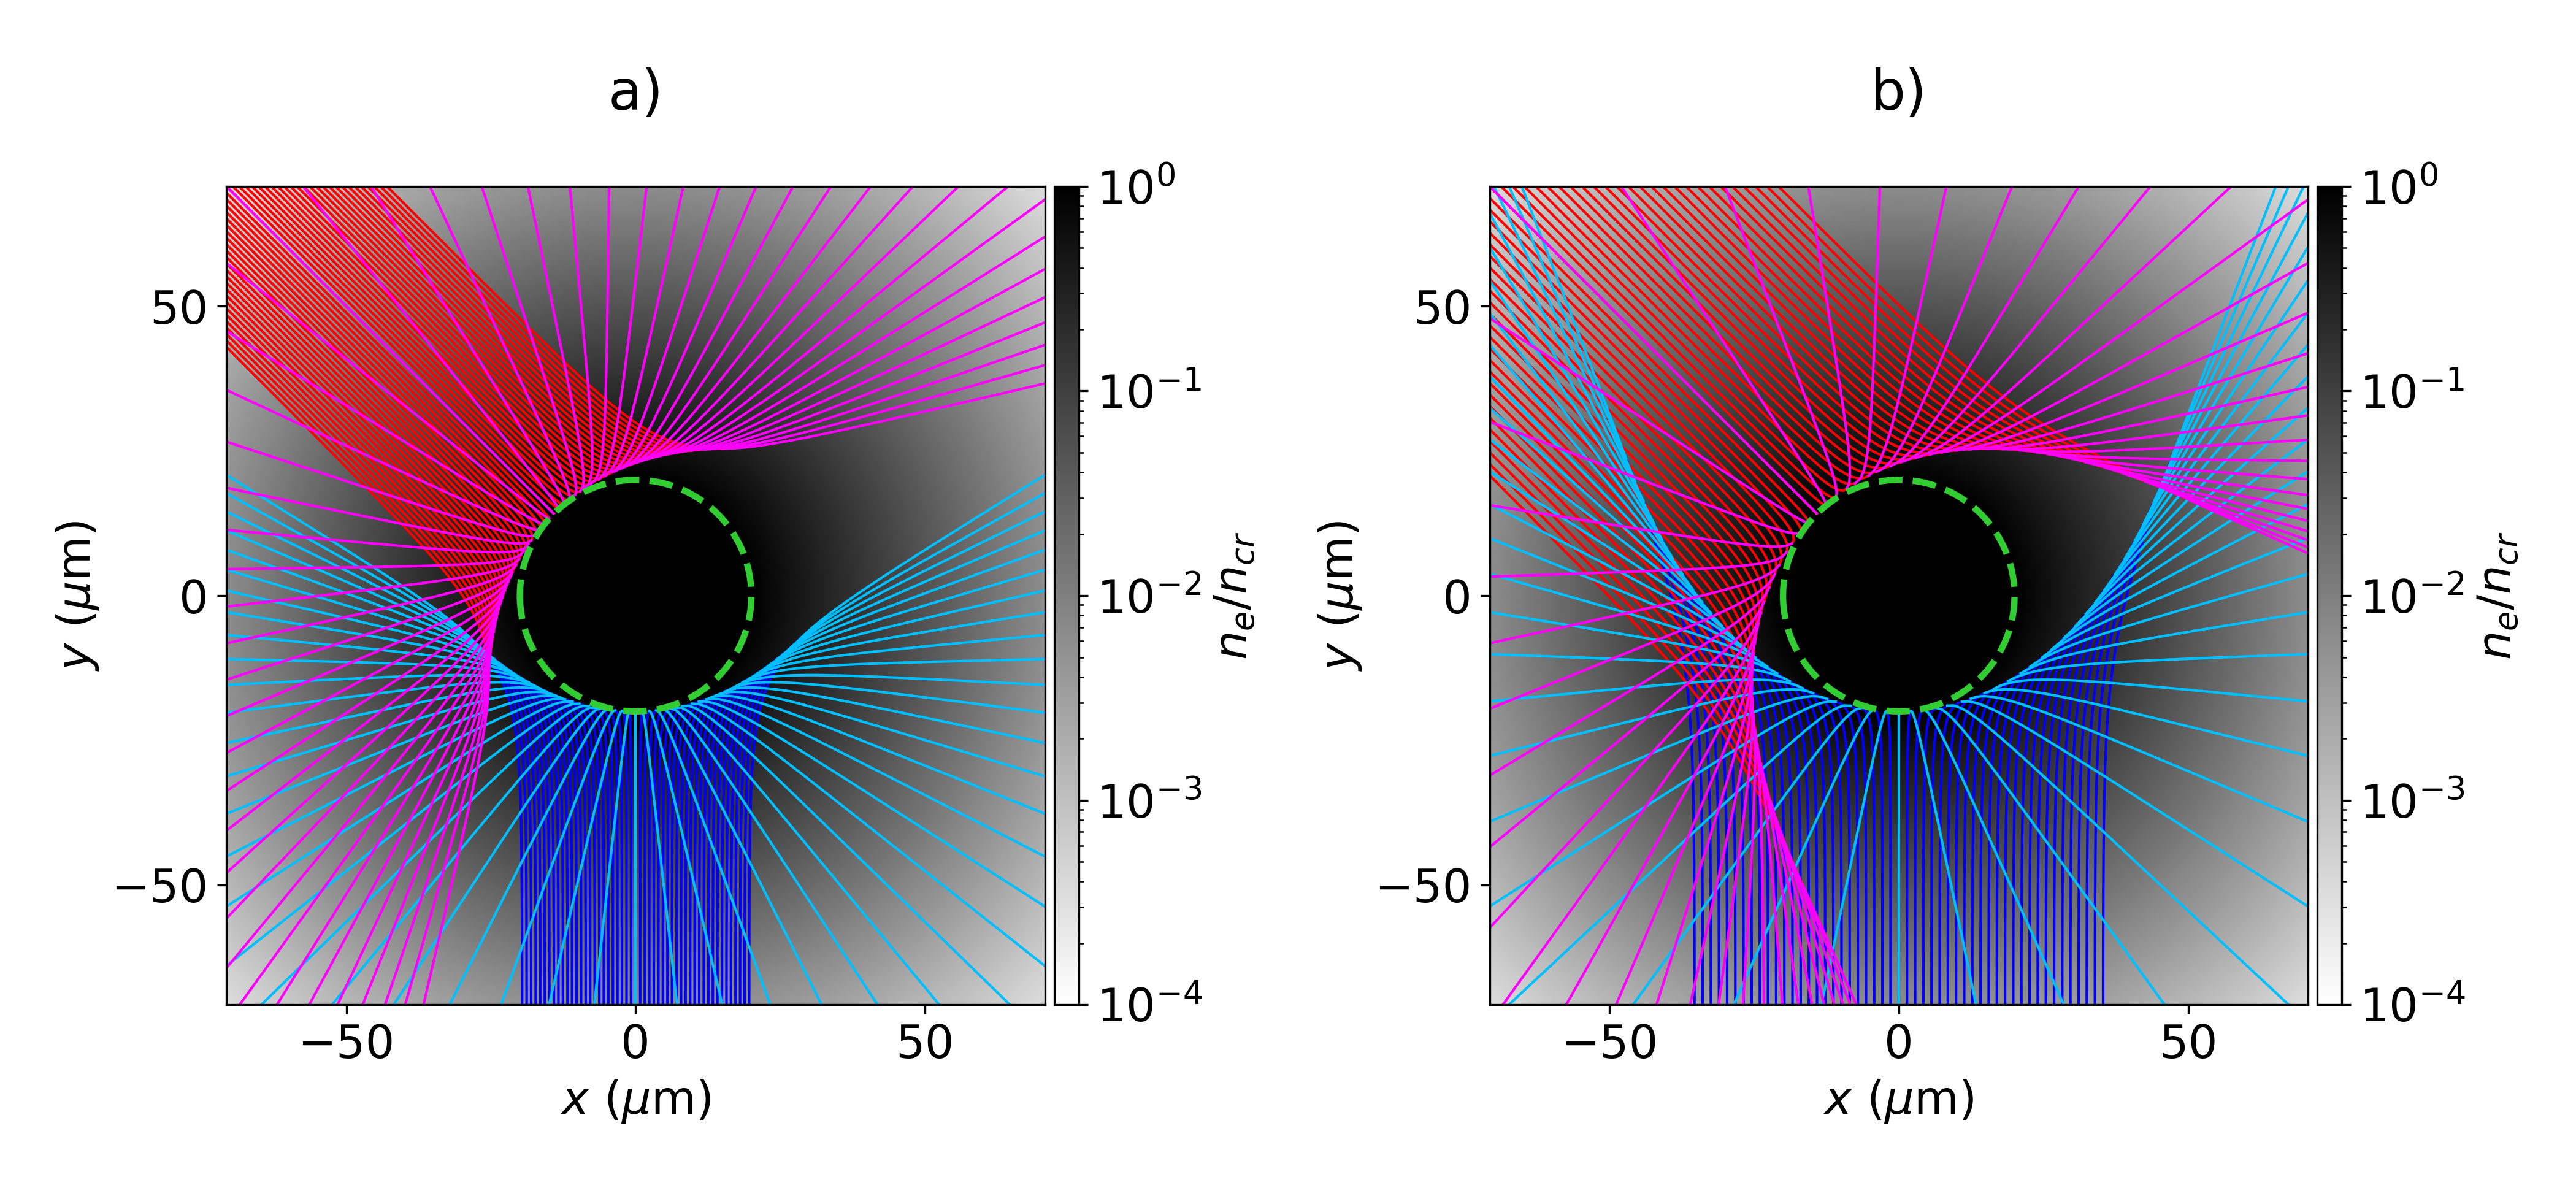
\includegraphics[width=\linewidth]{Results1/Images/RbRt_beam_overlap_alt.png}
    \centering
    \caption{The trajectory of rays from two beams with Beam radii.
    The density profile for both simulations is $n_e=n_{\text{cr}}\exp{[ -(r_{\mu\text{m}}-20)/100 ]}$.
    Panels a) and b) plot rays from beams with widths $\sigma=10$ and $18\ \mu\text{m}$ respectively.
    Ray trajectories are separated for each beam by colour depending on their sheet.
    Red and dark blue rays are from the incident sheet (before the ray caustic) and magenta and light blue rays are from the reflected sheet (after the ray caustic).}%
    \label{fig:Res1_RbRt_beam_overlap}
\end{figure}

An idealised direct drive implosion, (neglecting the effect of random or otherwise, shot-to-shot variations) has a limited number of initial conditions which define the implosion.
The target can be described by a set of materials and each of their thicknesses.
Initial target parameters are intimately coupled to the physics of the implosion and, in part, dictate the propagation time of shocks through the target, hydrodynamic stability and absorption of the laser energy.
The pulse shape describes the laser power which is incident of the target as a function of time, which itself can be parameterised by various features.
This can be altered to, for example, drive shocks by introducing sharp rises in the incident power with time.
A given facility also has a number of beam ports each of which has a specific origin and pointing location, which influence the magnitude of the \textit{beam mode} asymmetry, which arises from the uniformity of laser absorption.
The intensity profile of each laser and specifically the beam radius is an additional parameter which can be varied and plays an important role in defining both the power which can be coupled to the target and the magnitude of beam mode asymmetry.

At a specific laser facility, the ability to vary beam radius is often limited by the available optics, therefore it is often effectively varied from shot to shot by changing the outer radius of the target.
These parameters can then define a dimensional variable, which is the radius of the beam divided by the target radius.
Typically, at the \textsc{Omega} laser facility, this is explicitly defined as the radius of the beam which contains 95 \% of the incident power divided by the initial outer target radius,
\begin{equation}
    R_b/R_t = \frac{r_{95}}{R_t},
\end{equation}
where $r_{95}$ is defined by the integral,
\begin{equation}
    \int_0^{r_{95}}e^{- \left| \frac{r}{\sigma} \right| ^{n_s}}\text{d}r = 0.95,
\end{equation}
where the definition of a circular, super-Gaussian beam profile from Eq.~\ref{eq:supgaus} has been used.
In the absence of \ac{CBET} it can intuitively be understood that increasing this parameter should improve the uniformity of the laser illumination, because beam spots overlap each other more on the target, and therefore reduce the beam mode.
Larger $R_b/R_t$ also lead to slightly less absorption in the absence of \ac{CBET}, because a larger fraction of the incident light (especially at late time as the target converges) would reach lower density plasma and therefore not be absorbed.
\ac{CBET} significantly complicates this interpretation, however.

Fig.~\ref{fig:Res1_RbRt_beam_overlap}.a and Fig.~\ref{fig:Res1_RbRt_beam_overlap}.b plot results of a ray tracing calculation with a direct-drive relevant, exponentially decaying plasma density with a smaller and larger beam respectively.
In direct-drive, backscatter \ac{CBET} is the dominant mechanism which depletes absorption, which is where outbound light gains energy from inbound light\footnote{Note here that outbound here means light travelling quasi-parallel to the approximately radially outward fluid velocity and inbound means quasi-anti-parallel.}.
The outward rays from the small beam radius simulation in Fig.~\ref{fig:Res1_RbRt_beam_overlap}.a do not overlap the incident light from the other beam and therefore limited \ac{CBET} between these beams will occur.
The trajectories from the larger radius simulation in Fig.~\ref{fig:Res1_RbRt_beam_overlap}.b, however do cross the inbound rays from the other beam, which could lead to a resonant \ac{CBET} interaction, and significant reduction of the absorbed power.
As was shown in Fig.~\ref{fig:SOLAS_qpR_IFRIIT_test}, \ac{CBET} also substantially increases absorption asymmetry on the \textsc{Omega} laser facility.
This means that in the presence of \ac{CBET}, the effect of increasing $R_b/R_t$ on illumination asymmetry is not clear.
While in the absence of \ac{CBET}, it should lead to greater beam overlap, this increased overlap will result in more \ac{CBET} which could reduce uniformity of absorption.

Isolating the contribution of \ac{CBET} is of particular importance to allow extrapolation of experimental results to future facilities, because it is hoped that adding bandwidth to lasers will almost entirely eliminate \ac{CBET} scattering.
Studying which of these effects dominates is difficult to do experimentally, as significant backscatter \ac{CBET} occurs at all laser facilities which are capable of conducting compression experiments.
Therefore, computational studies are well suited to investigate how $R_b/R_t$ influences performance and the role of \ac{CBET} in this scaling.

%################################################################################
%################################################################################
\subsection{Statistical Modelling of \textsc{Omega} Direct-Drive Implosions}%
\label{sec:Res1_OMEGA_stat_modelling}


%################################################################################
%################################################################################
\subsection{Beam Radius in Statistical Modelling}%
\label{sec:Res1_OMEGA_stat_modelling_RbRt}


%###############################################################################################################################
%###############################################################################################################################
%###############################################################################################################################
\section{Cylindrical Simulation Platform for Beam Radius Parameter Scan}%
\label{sec:Res1_CylRbRt_platform}


%################################################################################
%################################################################################
\subsection{Assumptions and Validity of the Cylindrical Simulation Platform}%
\label{sec:Res1_platformvalidity}


%################################################################################
%################################################################################
\subsection{Problems with Traditional Methods of Investigating Beam Radius Parameter Computationally}%
\label{sec:Res1_computational_difficulties}


%################################################################################
%################################################################################
\subsection{Pulse Shape and Target Initial Conditions}%
\label{sec:Res1_initialconditions}

\begin{figure}[t!]
    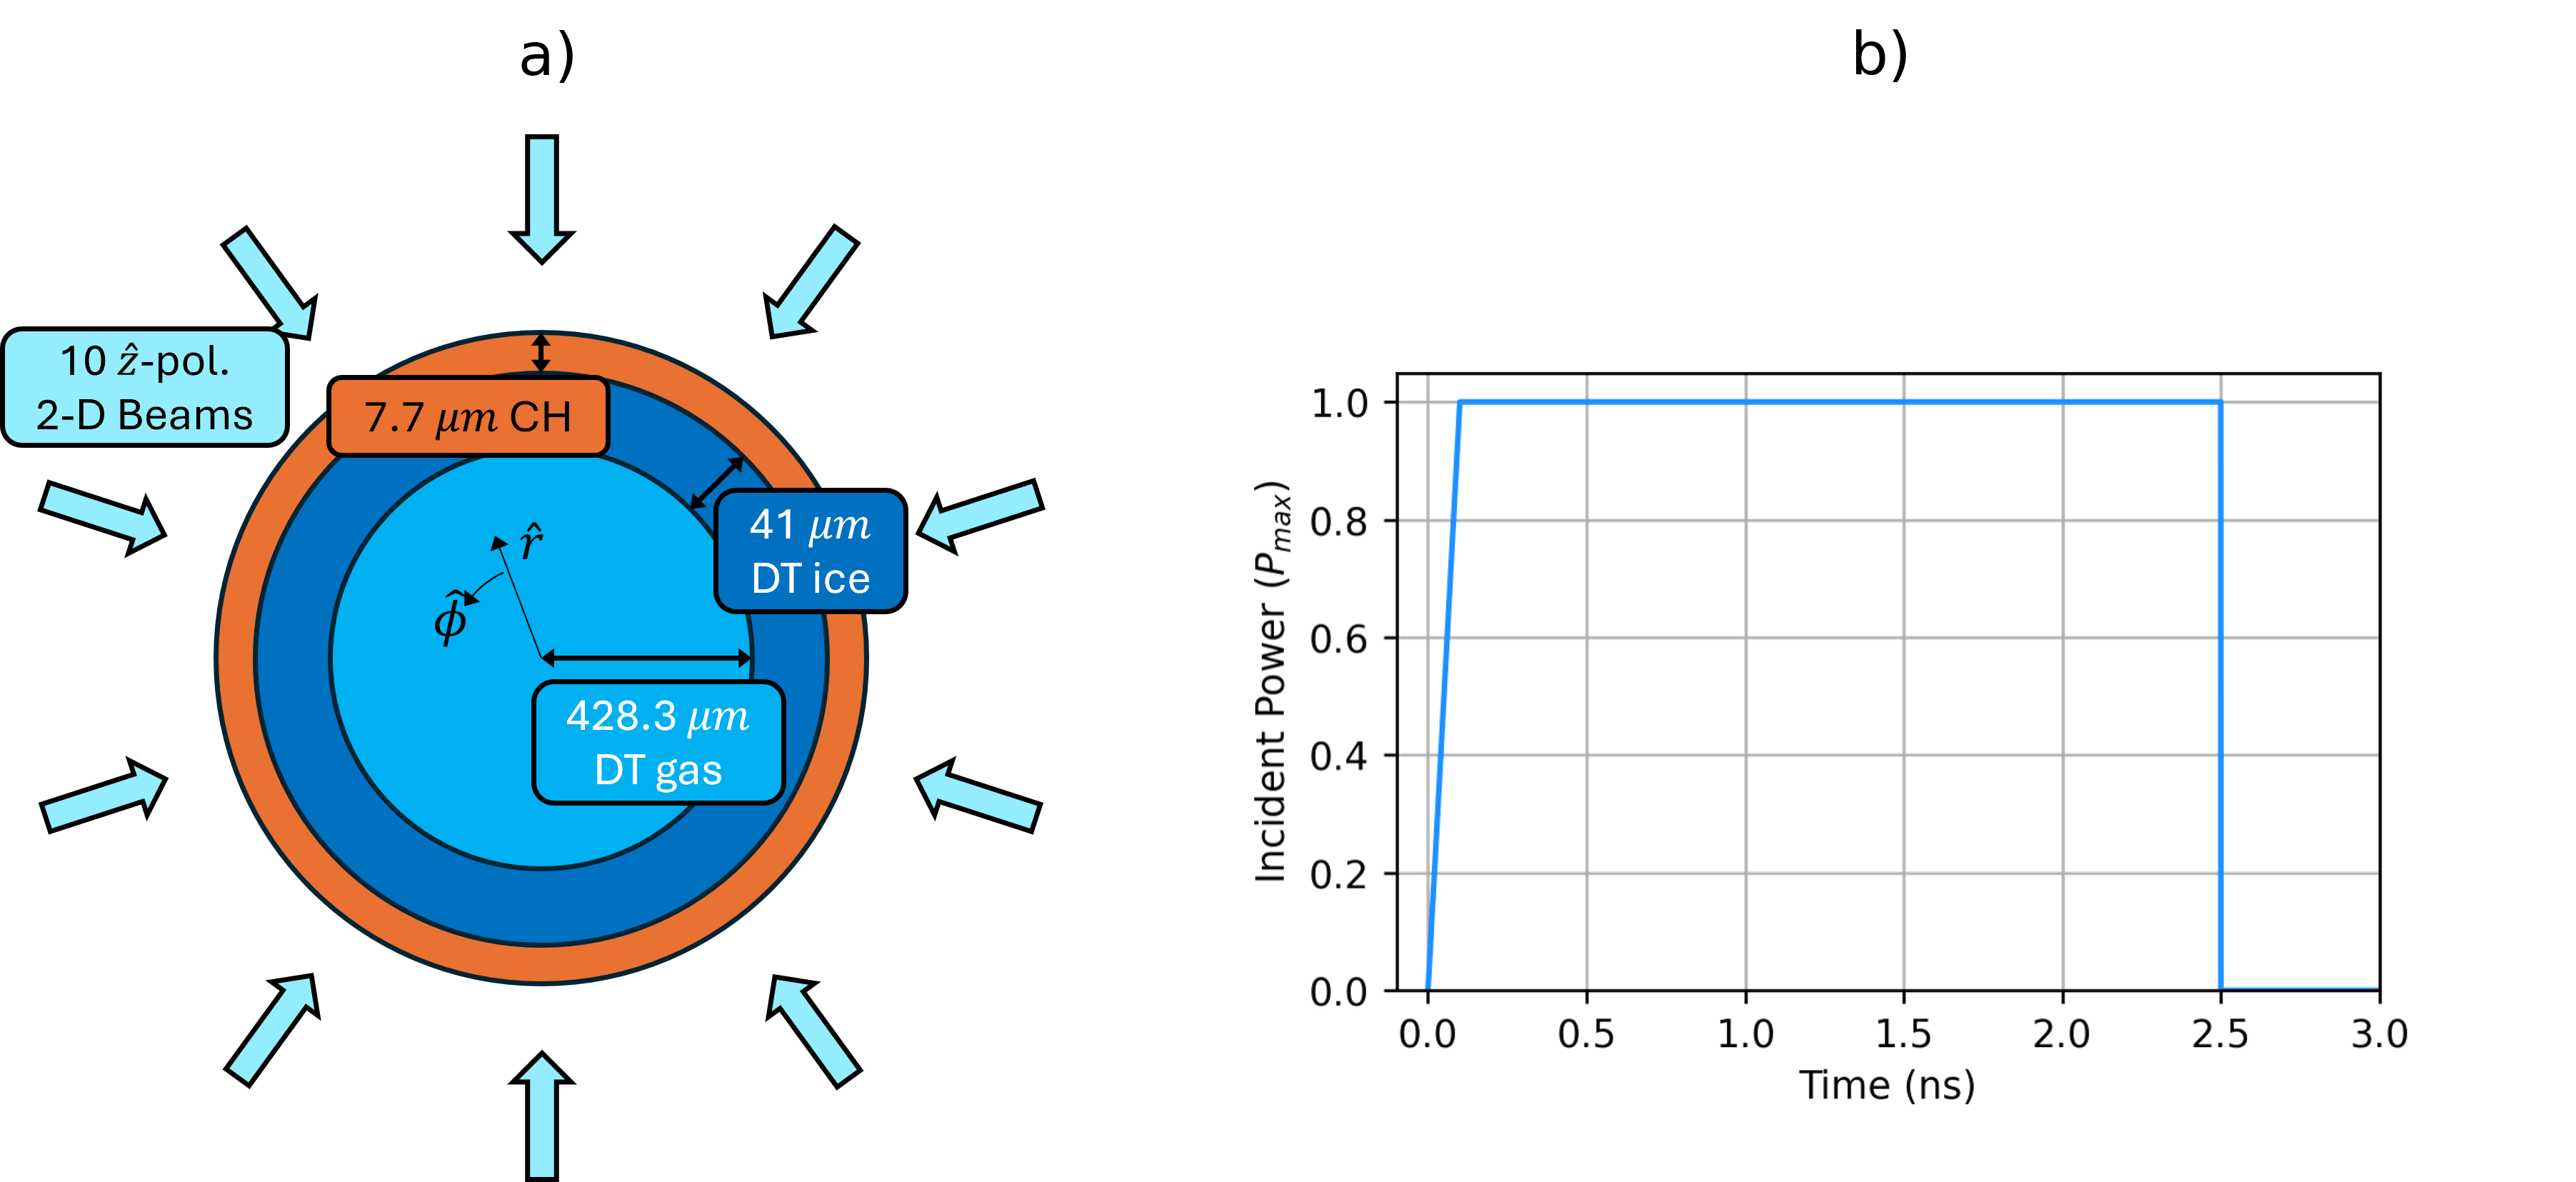
\includegraphics[width=\linewidth]{Results1/Images/cyl_setup.png}
    \centering
    \caption{The target initial conditions with beam geometry, a), and pulse shape, b), used for the 2-D cylindrical simulations.
    All beams were polarised out of the simulation plane, in the $+\hat{\vec{z}}$ direction.
    Initial layer radii were taken from the initial conditions for \textsc{Omega} shot 89224, presented in Fig.~\ref{fig:89224_ICs}.a.}%
    \label{fig:Res1_cyl_setup}
\end{figure}


%################################################################################
%################################################################################
\subsection{1-D Implosion Tuning}%
\label{sec:Res1_1D_tuning}

\bgroup
\def\arraystretch{1.2}%  1 is the default, change whatever you need
% Please add the following required packages to your document preamble:
% \usepackage{multirow}
\begin{table}[]
    \centering
    \caption{Results of the 1-D Tuning Simulations.}
    \begin{tabular}{cccccc}
    \hhline{======}
    $R_b/R_t$             &         & \begin{tabular}[c]{@{}c@{}}$P_{\text{max}}$\\ ($\text{TW}/\text{cm}$)\end{tabular} & \begin{tabular}[c]{@{}c@{}}$I_0$\\ ($10^{14}\ \text{W}/\text{cm}^2$)\end{tabular} & \begin{tabular}[c]{@{}c@{}}$t_{\text{bang}}$\\ ($\text{ns}$)\end{tabular} & \begin{tabular}[c]{@{}c@{}}$Y_{\text{DT}}$\\ ($10^{13}\ /\text{cm}$)\end{tabular} \\ \hhline{======}
    \multirow{2}{*}{0.75} & No CBET & \multirow{2}{*}{54.44}                                                             & \multirow{2}{*}{0.85}                                                   & 2.49                                                                      & 1.53                                 \\
                          & CBET    &                                                                                    &                                                                         & 2.51                                                                      & 1.44                                 \\ \hline
    \multirow{2}{*}{0.80} & No CBET & \multirow{2}{*}{58.25}                                                             & \multirow{2}{*}{0.83}                                                   & 2.49                                                                      & 1.56                                 \\
                          & CBET    &                                                                                    &                                                                         & 2.51                                                                      & 1.45                                 \\ \hline
    \multirow{2}{*}{0.85} & No CBET & \multirow{2}{*}{63.44}                                                             & \multirow{2}{*}{0.83}                                                   & 2.48                                                                      & 1.67                                 \\
                          & CBET    &                                                                                    &                                                                         & 2.51                                                                      & 1.43                                 \\ \hline
    \multirow{2}{*}{0.90} & No CBET & \multirow{2}{*}{70.00}                                                             & \multirow{2}{*}{0.85}                                                   & 2.47                                                                      & 1.82                                 \\
                          & CBET    &                                                                                    &                                                                         & 2.50                                                                      & 1.41                                 \\ \hline
    \multirow{2}{*}{0.95} & No CBET & \multirow{2}{*}{77.94}                                                             & \multirow{2}{*}{0.89}                                                   & 2.46                                                                      & 1.99                                 \\
                          & CBET    &                                                                                    &                                                                         & 2.49                                                                      & 1.49                                 \\ \hline
    \multirow{2}{*}{1.00} & No CBET & \multirow{2}{*}{87.25}                                                             & \multirow{2}{*}{0.93}                                                   & 2.45                                                                      & 2.15                                 \\
                          & CBET    &                                                                                    &                                                                         & 2.49                                                                      & 1.60                                 \\ \hline
    \multirow{2}{*}{1.05} & No CBET & \multirow{2}{*}{97.94}                                                             & \multirow{2}{*}{0.99}                                                   & 2.46                                                                      & 2.27                                 \\
                          & CBET    &                                                                                    &                                                                         & 2.50                                                                      & 1.61                                 \\ \hline
    \multirow{2}{*}{1.10} & No CBET & \multirow{2}{*}{110.00}                                                            & \multirow{2}{*}{1.06}                                                   & 2.47                                                                      & 2.31                                 \\
                          & CBET    &                                                                                    &                                                                         & 2.51                                                                      & 1.52                                 \\ \hhline{======}
    \end{tabular}
    \label{tab:res1_1d_tuning}
\end{table}
\egroup

\begin{figure}[t!]
    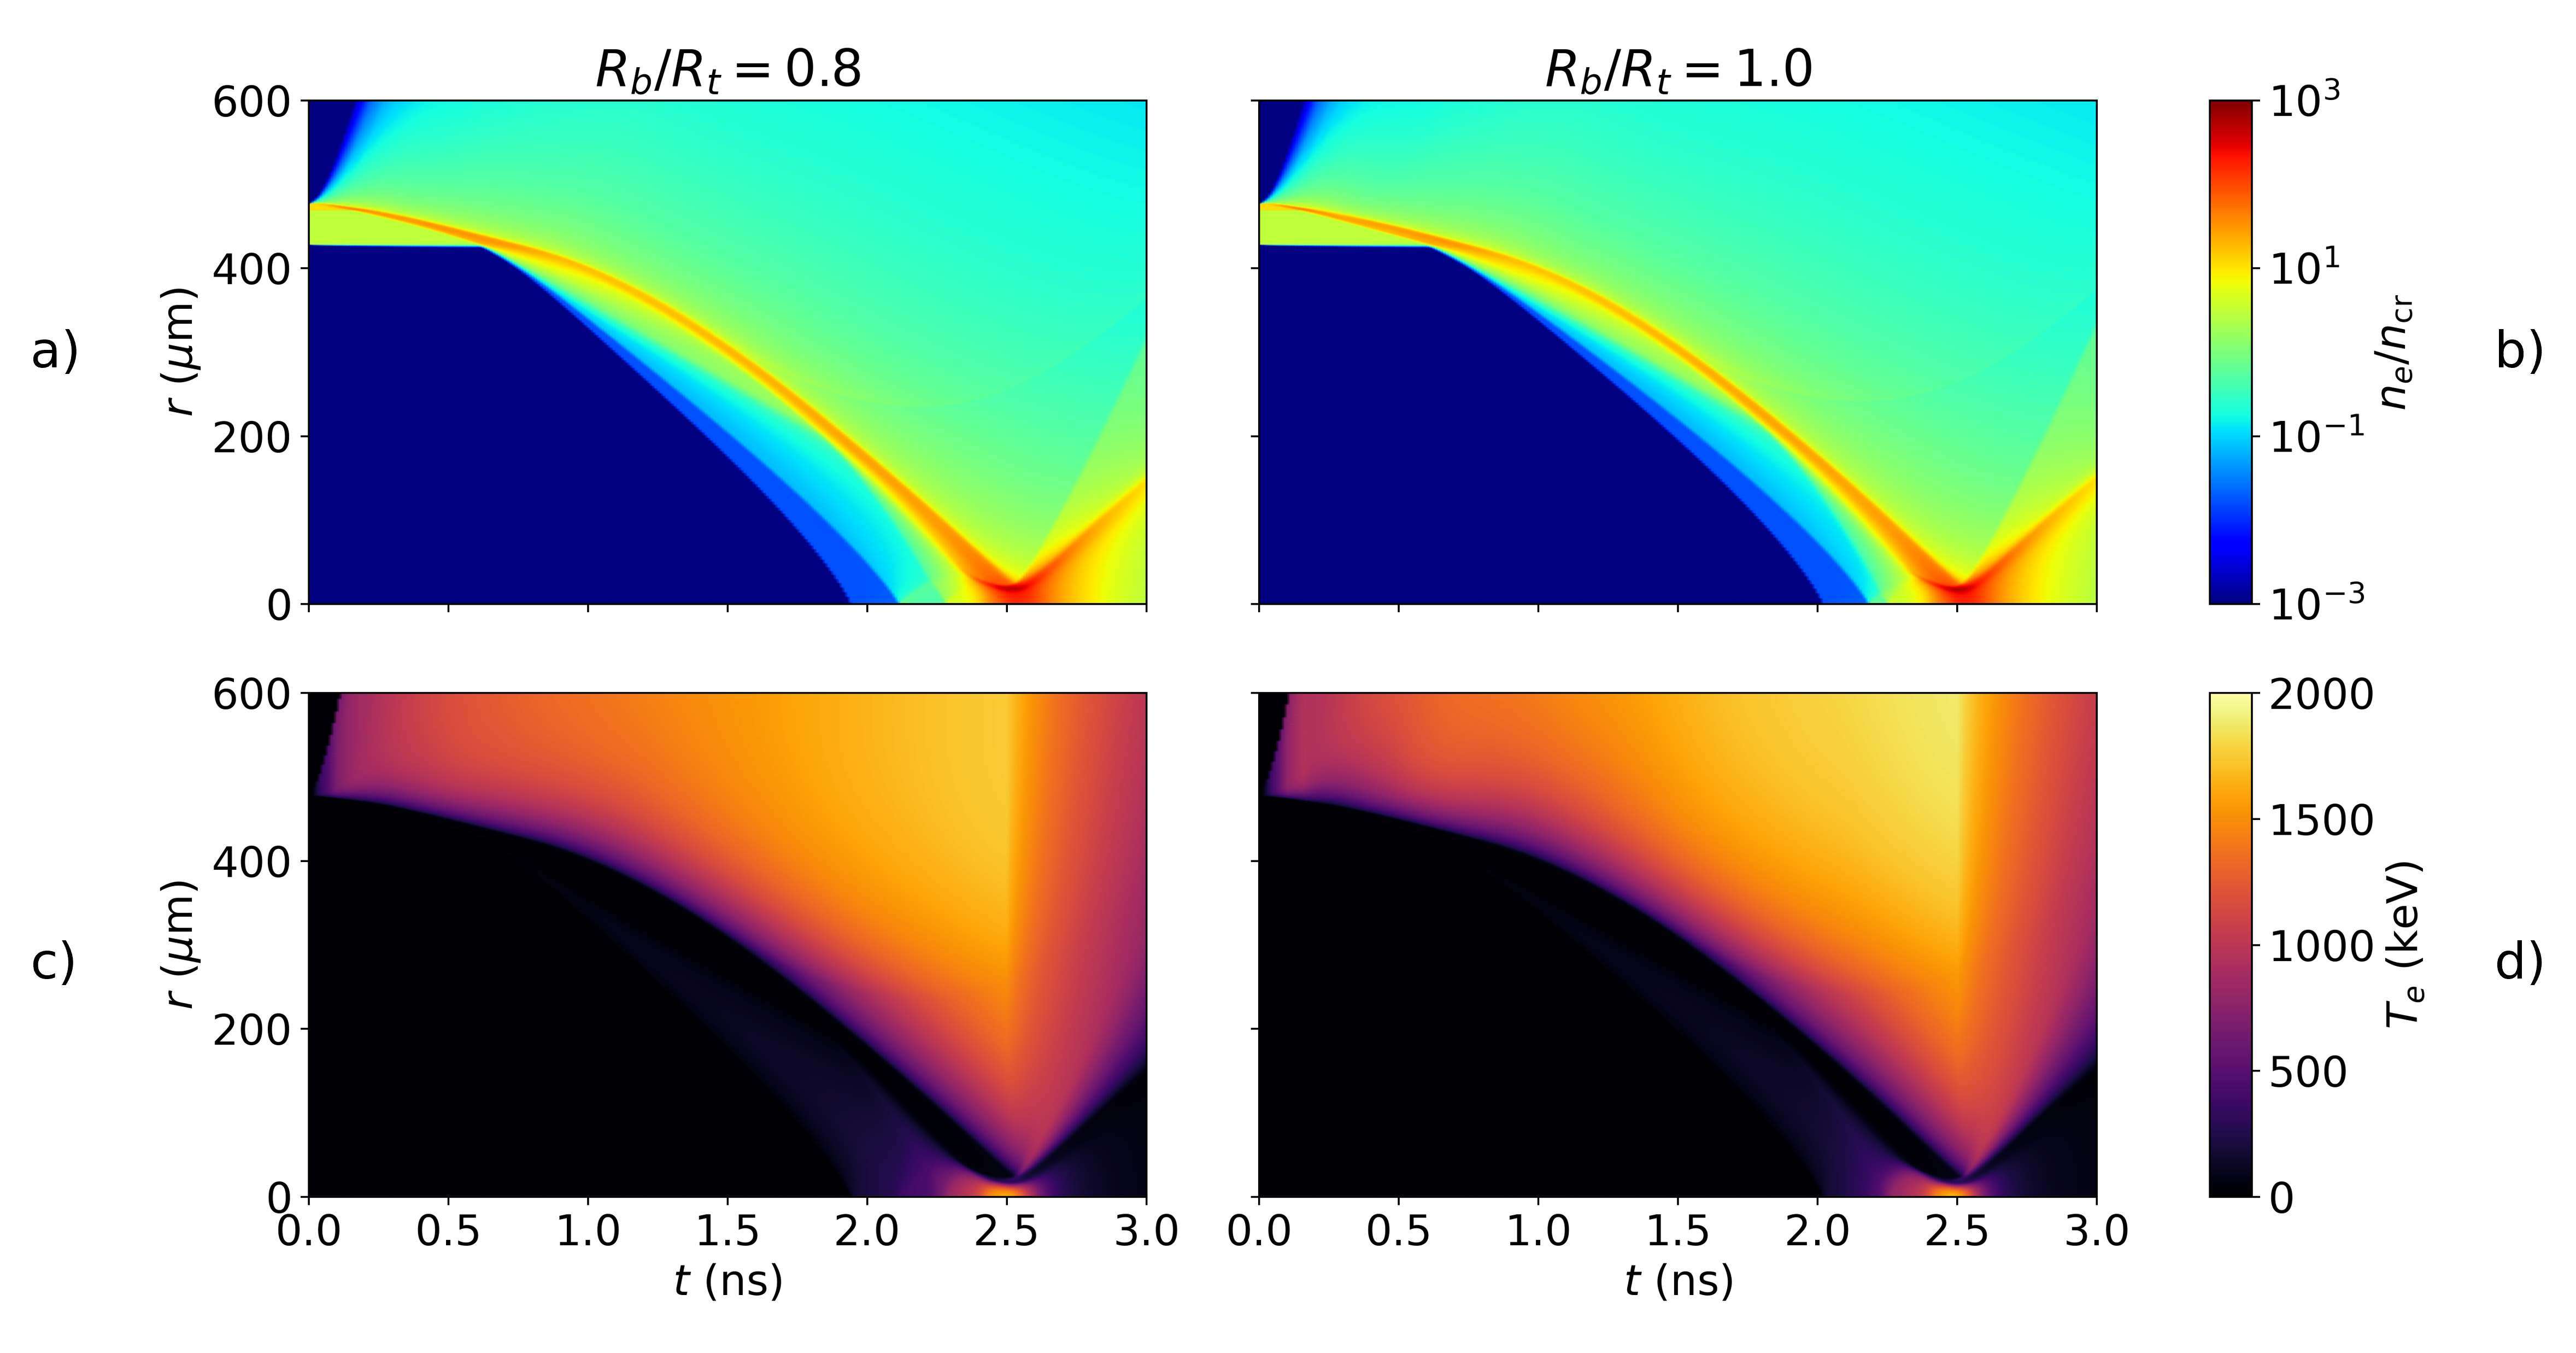
\includegraphics[width=\linewidth]{Results1/Images/streaks.png}
    \centering
    \caption{Streak plots from two of the 1-D tuning simulations.
    Panels a) \& b) plot the electron density as a function of time ($x$-axis) and radius ($y$-axis) for the \ac{CBET} simulations of the $R_b/R_t=0.8$ \& $R_b/R_t=1.0$ simulations respectively.
    Panels c) \& d) plot the same but electron temperature for the $R_b/R_t=0.8$ \& $R_b/R_t=1.0$ simulations respectively.}%
    \label{fig:Res1_streaks}
\end{figure}


%###############################################################################################################################
%###############################################################################################################################
%###############################################################################################################################
\section{CBET Induced Modal Flips in Power Deposition Asymmetries}%
\label{sec:Res1_PdepR_CBET_asymm}


%################################################################################
%################################################################################
\subsection{Analysis and Quantity Definitions}%
\label{sec:Res1_analysis_and_def}

\begin{figure}[t!]
    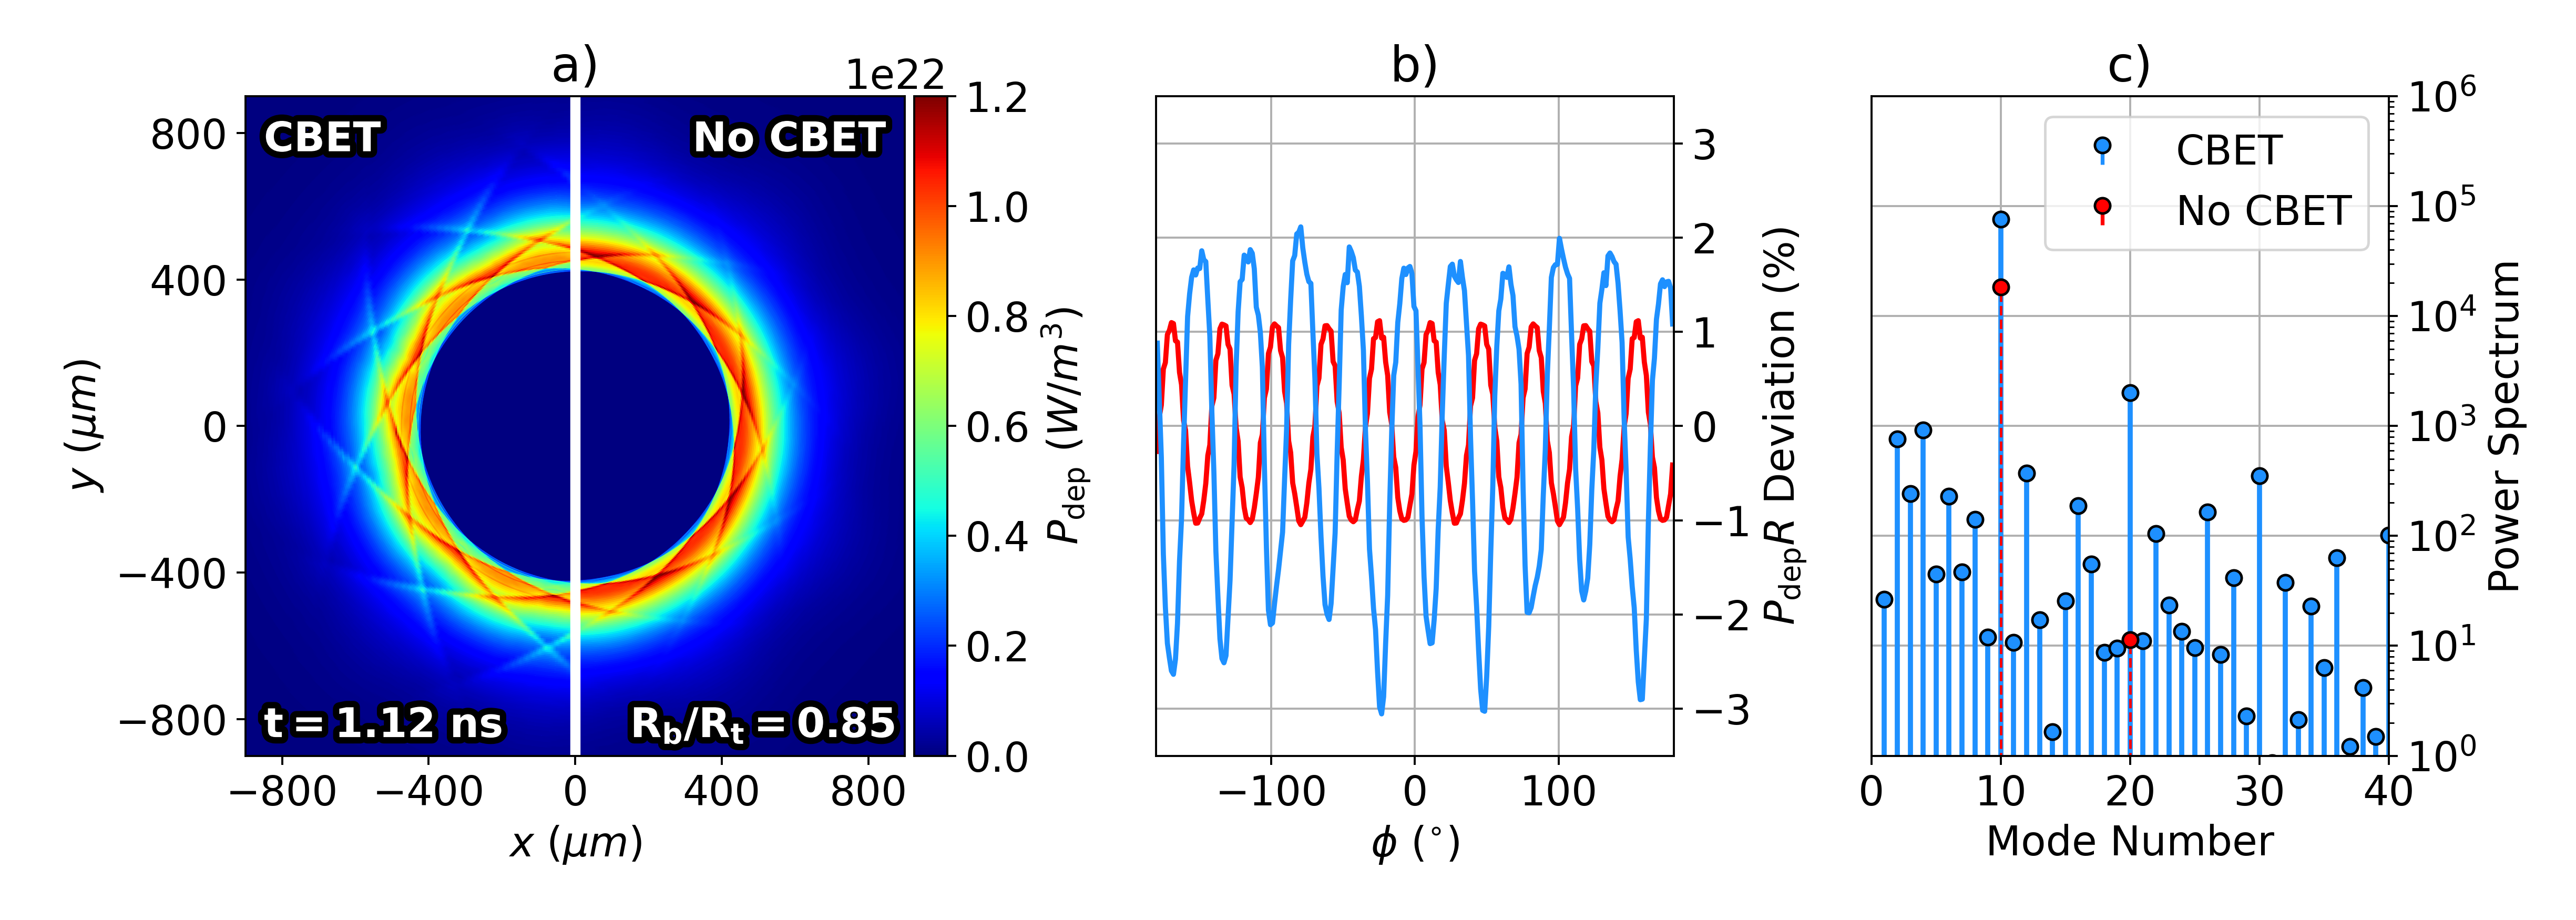
\includegraphics[width=\linewidth]{Results1/Images/Mode_analysis.png}
    \centering
    \caption{This figure demonstrates the analysis workflow to obtain the key results for this chapter.
    The power deposition at $t=1.12\ \text{ns}$ from the \ac{CBET} (left) and no \ac{CBET} (right) simulations are plotted in panel a) for the $R_b/R_t=0.85$ case.
    Panel b) plots the radially integrated deposition from the profiles in a) as a function of azimuthal angle.
    It can be seen from this plot, that the \ac{CBET} asymmetry (light-blue) is greater than the no \ac{CBET} asymmetry (red).
    The power spectrum of these profiles is then plotted in panel c).
    This demonstrates that the dominant modes in the spectrum are multiples of the number of beams.}%
    \label{fig:Res1_analysis}
\end{figure}


%################################################################################
%################################################################################
\subsection{Deposition Asymmetries in the Absence of CBET}%
\label{sec:Res1_noCBET_asymmetries}

\begin{figure}[t!]
    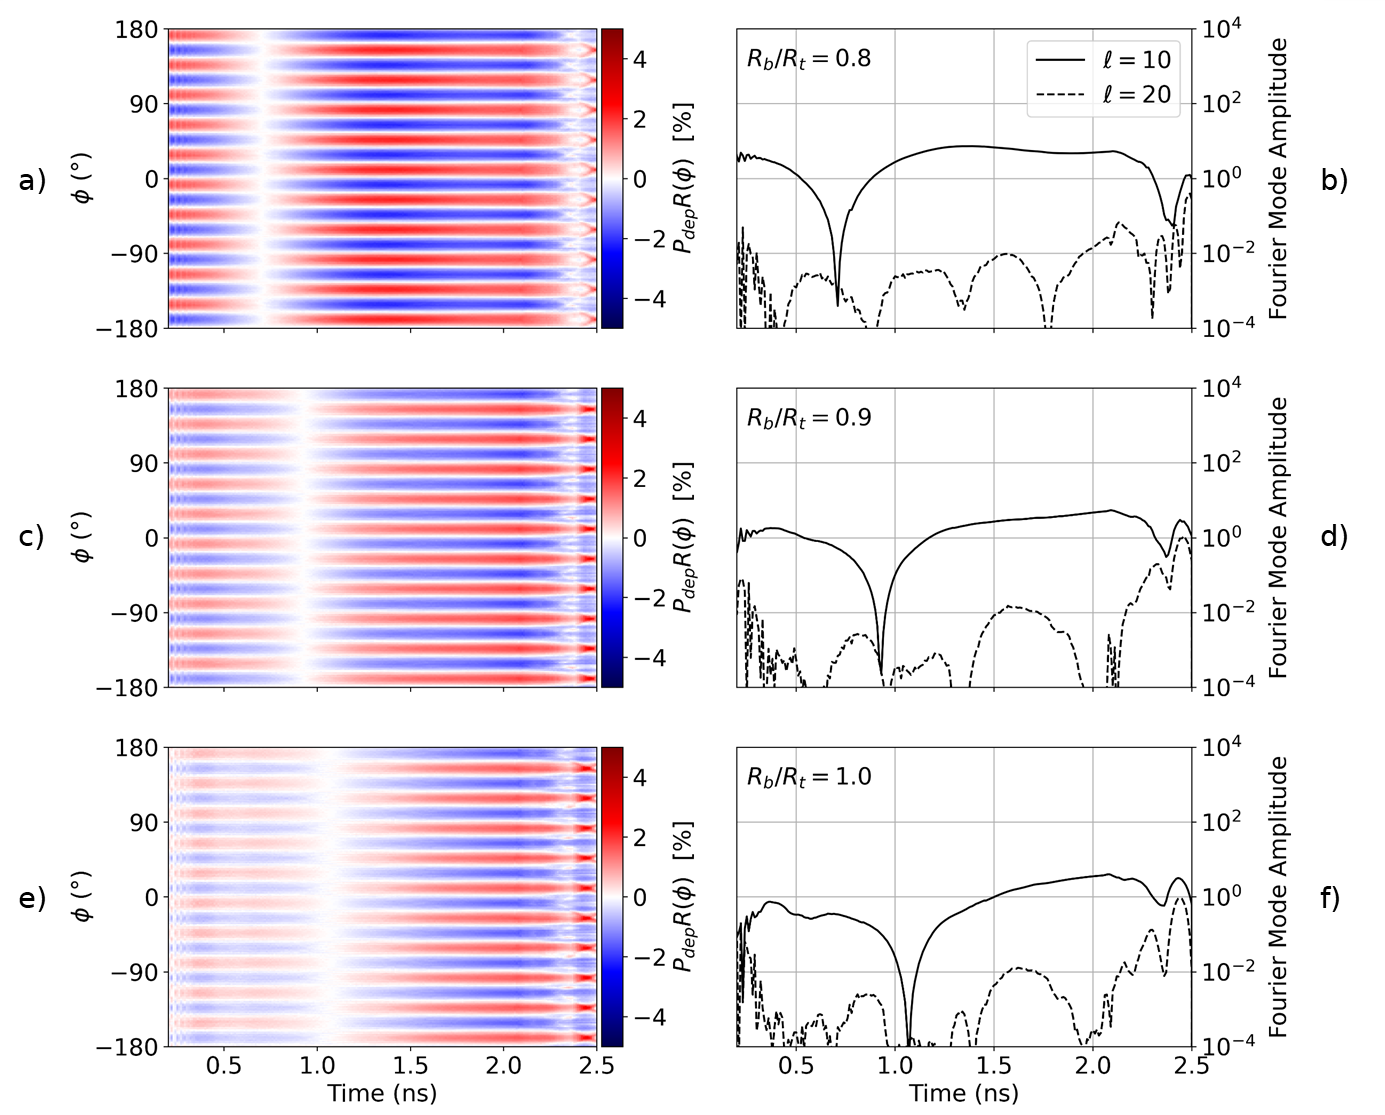
\includegraphics[width=\linewidth]{Results1/Images/noCBET_PR_modes.png}
    \centering
    \caption{This figure plots the radially integrated deposited power from no \ac{CBET} simulations as a function of time ($x$-axis) and angle ($y$-axis), alongside amplitudes of the dominant modes from a Fourier power spectrum.
    Panels a) and b) plot the radially integrated deposited power and Fourier modes respectively for the $R_b/R_t=0.8$ simulation.
    The same is plotted for the $R_b/R_t=0.9$ simulation in c) \& d) and for the $R_b/R_t=1.0$ simulation in e) \& f).
    The mode 10 from the number of beams is clearly visible in the radially integrated power plots as 10 peaks to troughs in angle at a given time, \textit{i.e.} 10 cyclical perturbations along a vertical lineout.}%
    \label{fig:Res1_PR_noCBET_modes}
\end{figure}


%################################################################################
%################################################################################
\subsection{CBET Imprint on Incident Field}%
\label{sec:Res1_CBET_imprint}

\begin{figure}[t!]
    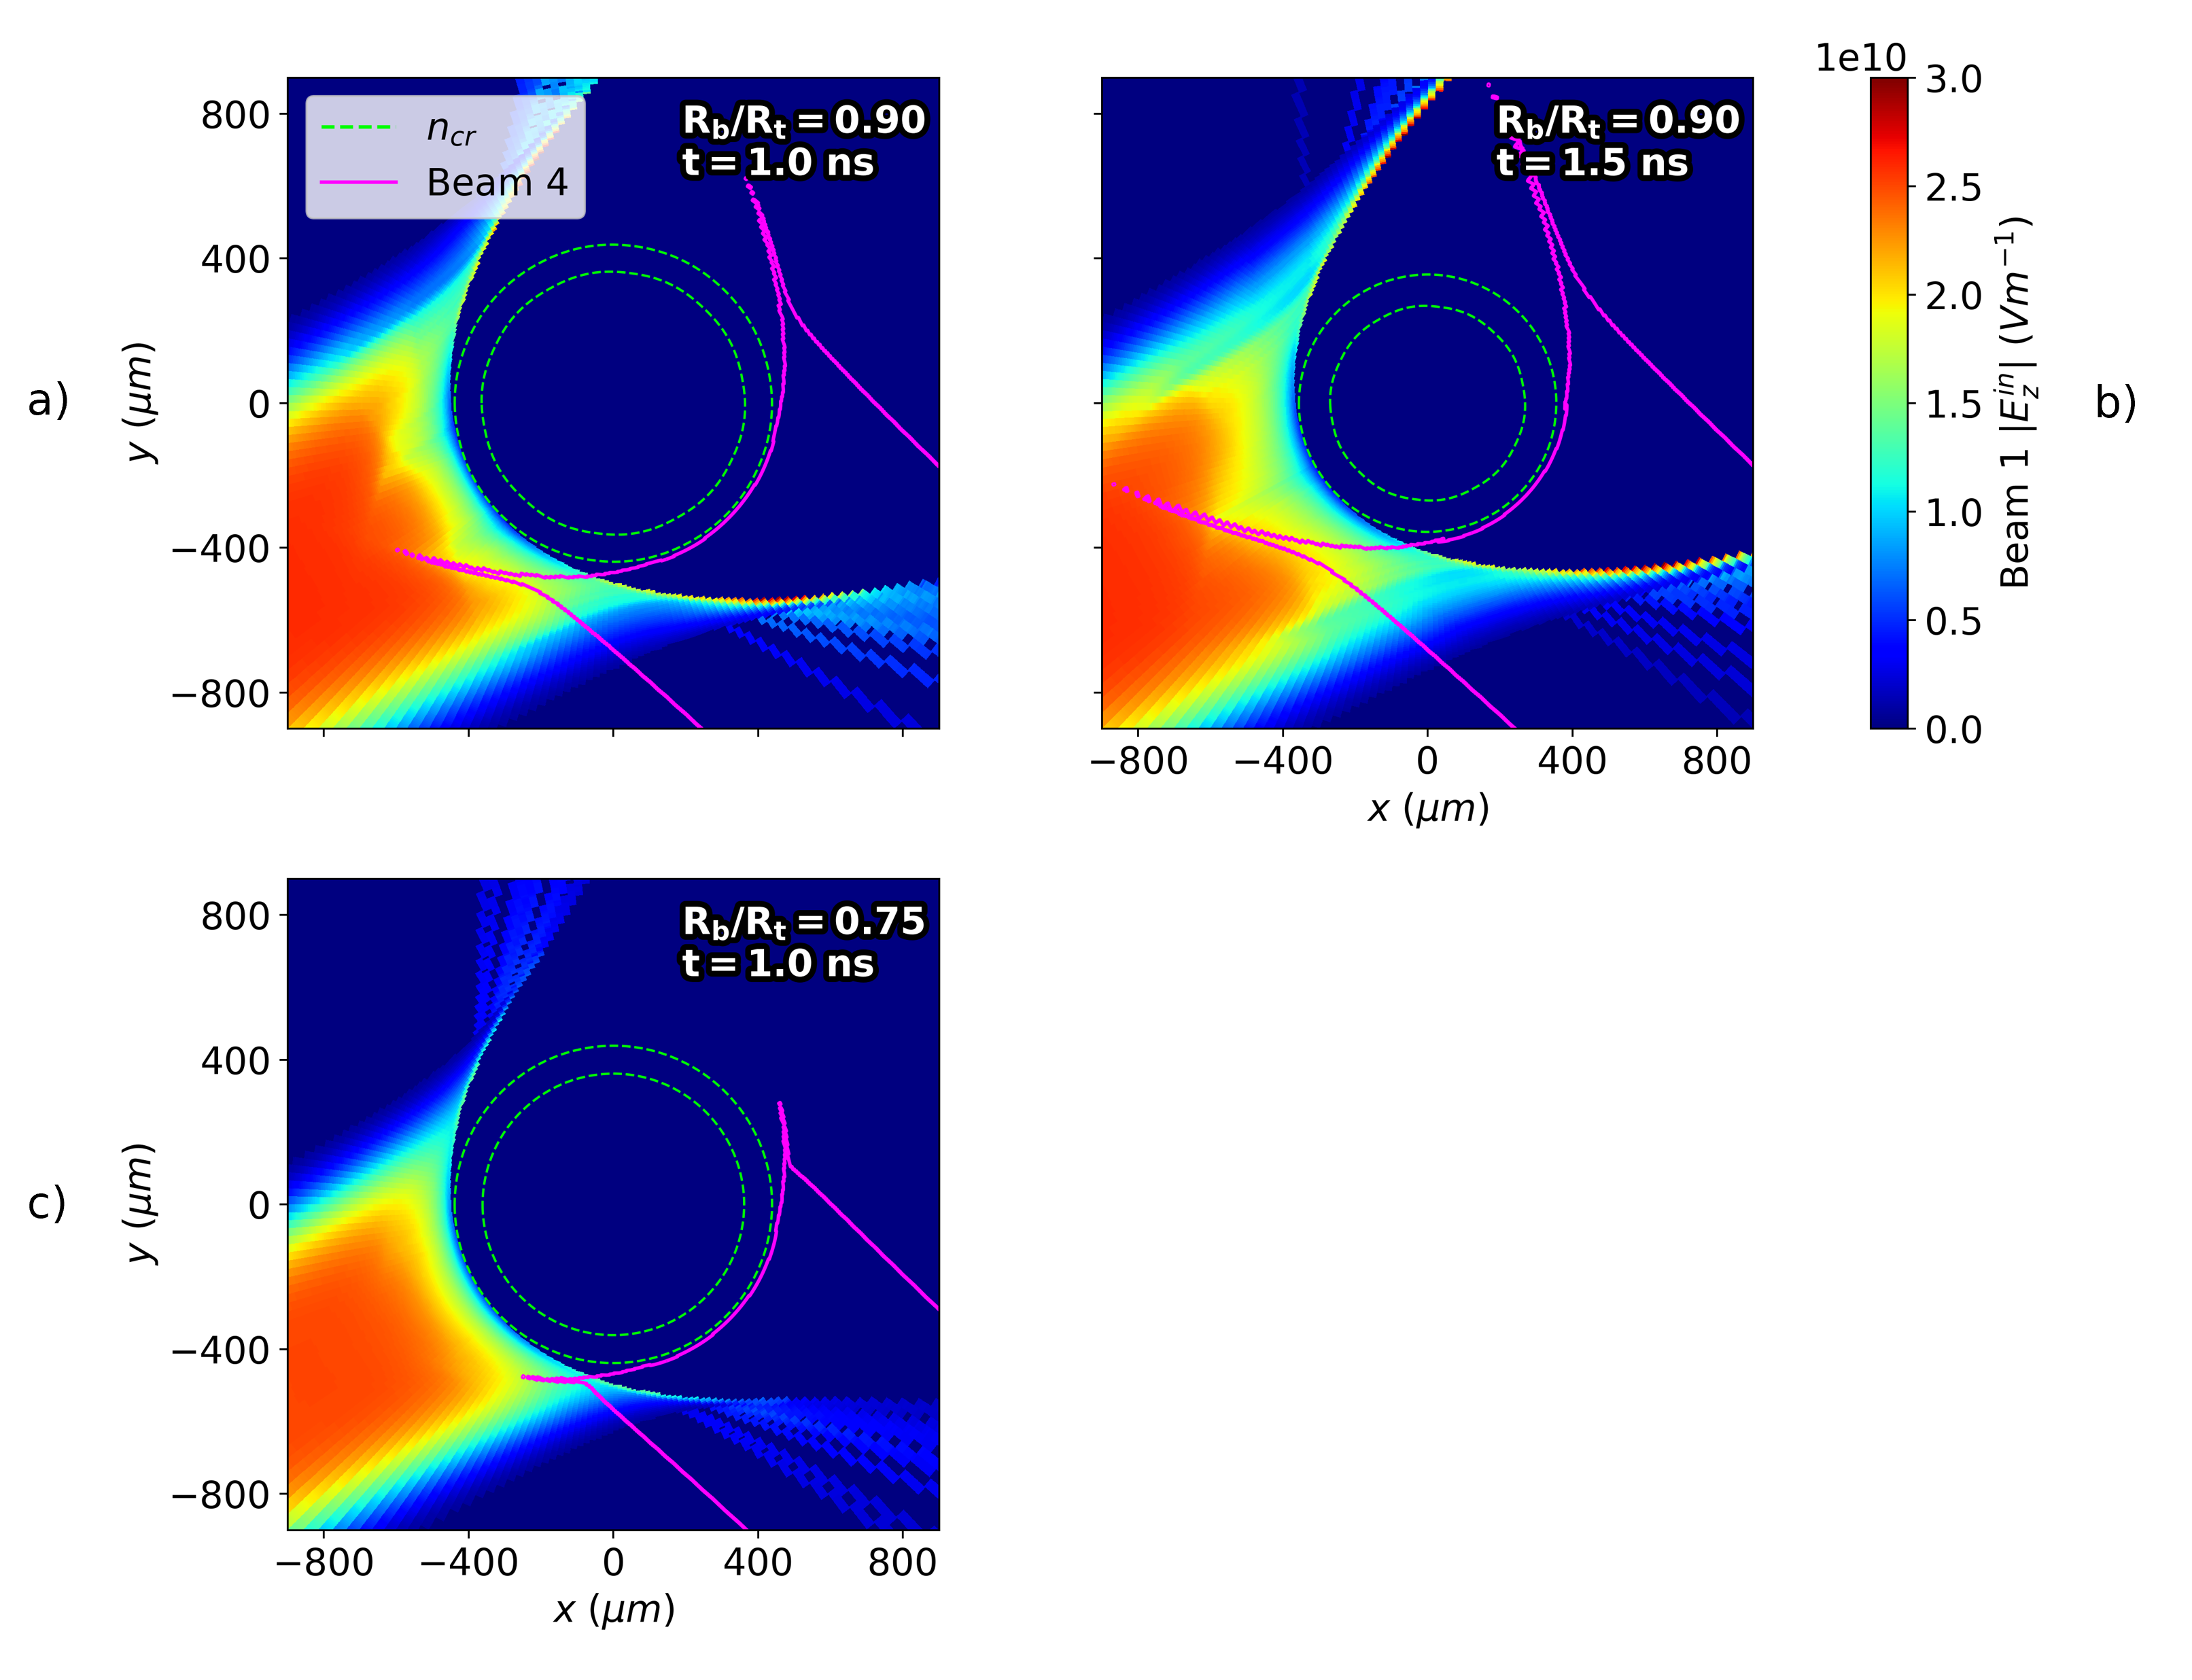
\includegraphics[width=\linewidth]{Results1/Images/Field_profiles.png}
    \centering
    \caption{This plot illustrates the origin of the \ac{CBET} induced asymmetry on power deposition and its dependence on $R_b/R_t$ and target convergence.
    Each panel plots the incident field (including the effect of \ac{CBET}), along with contours of the critical electron density and the $|E_z^{\text{in}}|=1\times10^{10}\ \text{Vm}^{-1}$ contour of another beam.
    Panel a) \& b) plot this for the $R_b/R_t=0.9$ simulation at $t=1.0\ \text{ns}$ \& $t=1.5\ \text{ns}$ respectively.
    The convergence of the target in this time interval leads to greater convergence and therefore a change in the spatial location across the beam of the resonant \ac{CBET} interaction.
    Panel c) plots the $R_b/R_t=0.75$ at the same time as panel a).
    This demonstrates that the $R_b/R_t=0.75$ beam is not wide enough at this time to lead to a resonant \ac{CBET} interaction, unlike the wider beam in panel a).}%
    \label{fig:Res1_field_profiles}
\end{figure}


%################################################################################
%################################################################################
\subsection{Modal Flips of Power Deposition Asymmetries}%
\label{sec:Res1_ModalFlip}

\begin{figure}[t!]
    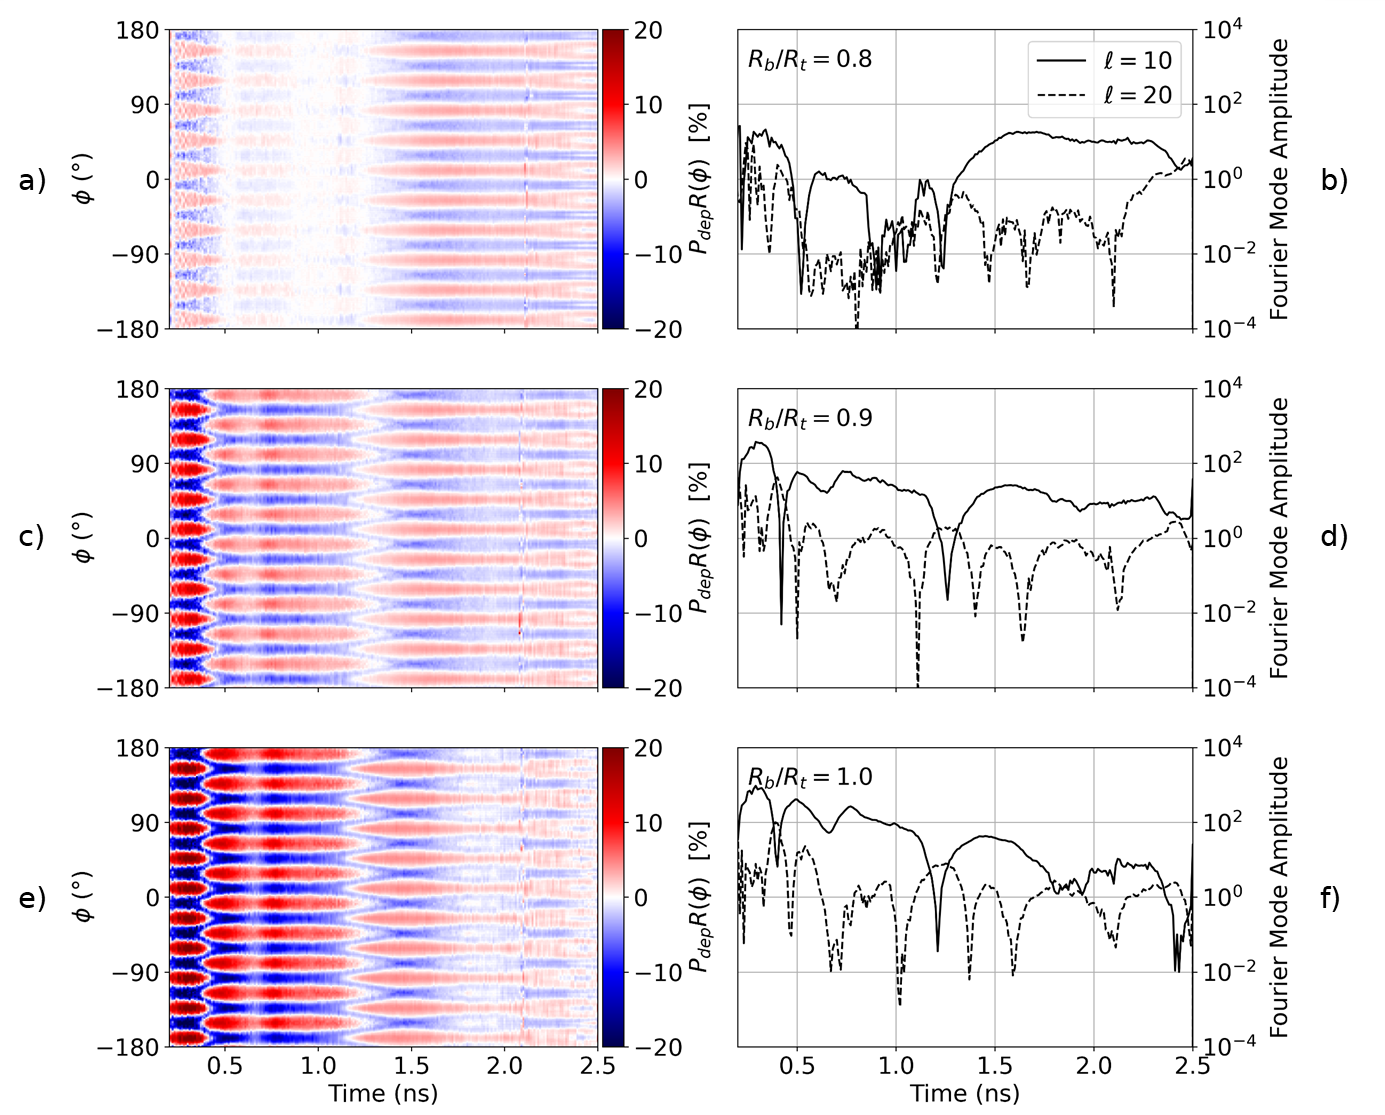
\includegraphics[width=\linewidth]{Results1/Images/CBET_PR_modes.png}
    \centering
    \caption{This figure plots the same as Fig.~\ref{fig:Res1_PR_noCBET_modes}, but now for the equivalent simulation including the effect of \ac{CBET}.
    Comparing these results and those in Fig.~\ref{fig:Res1_PR_noCBET_modes} demonstrates that \ac{CBET} introduces additional modal-flips of the deposition and amplifies the magnitude of asymmetries.}%
    \label{fig:Res1_PR_CBET_modes}
\end{figure}


%###############################################################################################################################
%###############################################################################################################################
%###############################################################################################################################
\section{Stagnation State Asymmetry}%
\label{sec:Res1_StagnationAsymm}


%################################################################################
%################################################################################
\subsection{Hotspot Profiles}%
\label{sec:Res1_HS_profiles}

\begin{figure}[t!]
    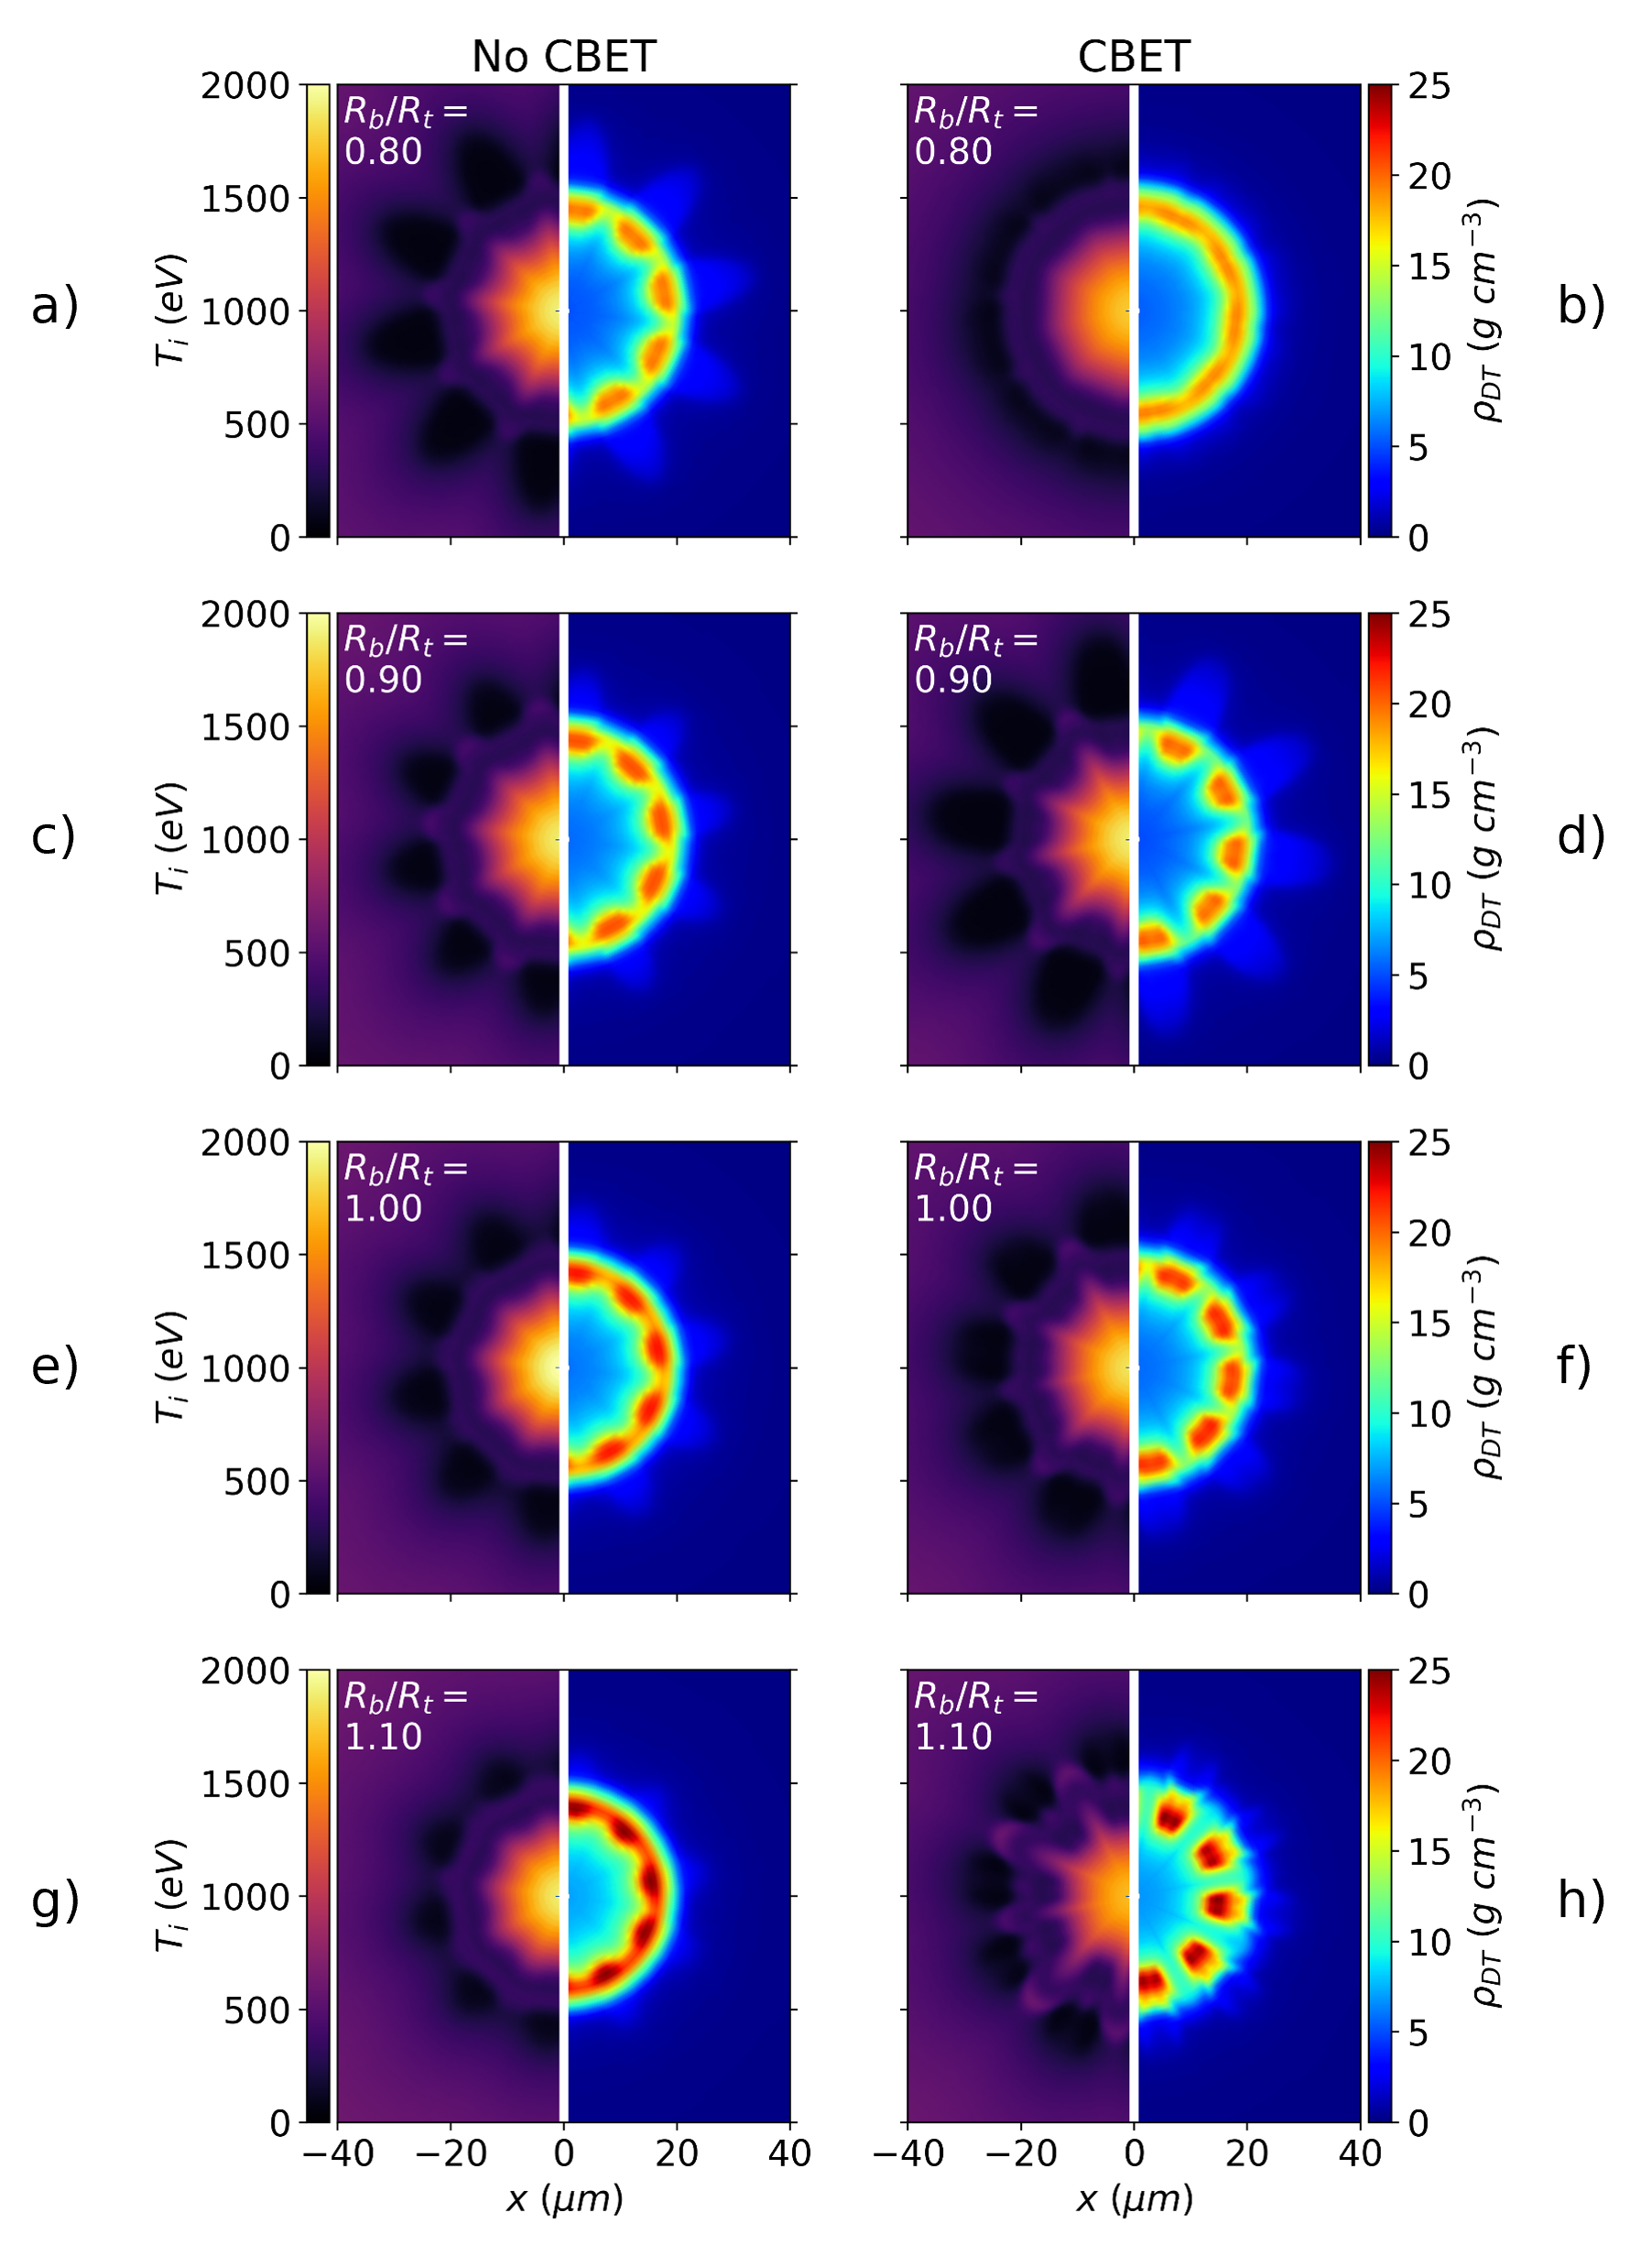
\includegraphics[width=0.9\linewidth]{Results1/Images/Stagnation_plots.png}
    \centering
    \caption{Densities of the DT fuel and ion temperatures for various $R_b/R_t$ simulations both with and without \ac{CBET}.
    Each row correspond to a different $R_b/R_t$ value; the left column contains simulations without \ac{CBET}; and the right column contains simulations with \ac{CBET}.
    It is visible from the density plots that increasing $R_b/R_t$ improves stagnation symmetry for the no \ac{CBET} simulations, but degrades it for the \ac{CBET} simulations.}%
    \label{fig:Res1_stagnation_plots}
\end{figure}



%################################################################################
%################################################################################
\subsection{Stagnation State Asymmetry Trend with Beam Radius}%
\label{sec:Res1_stagnation_asymm_trend}

\begin{figure}[t!]
    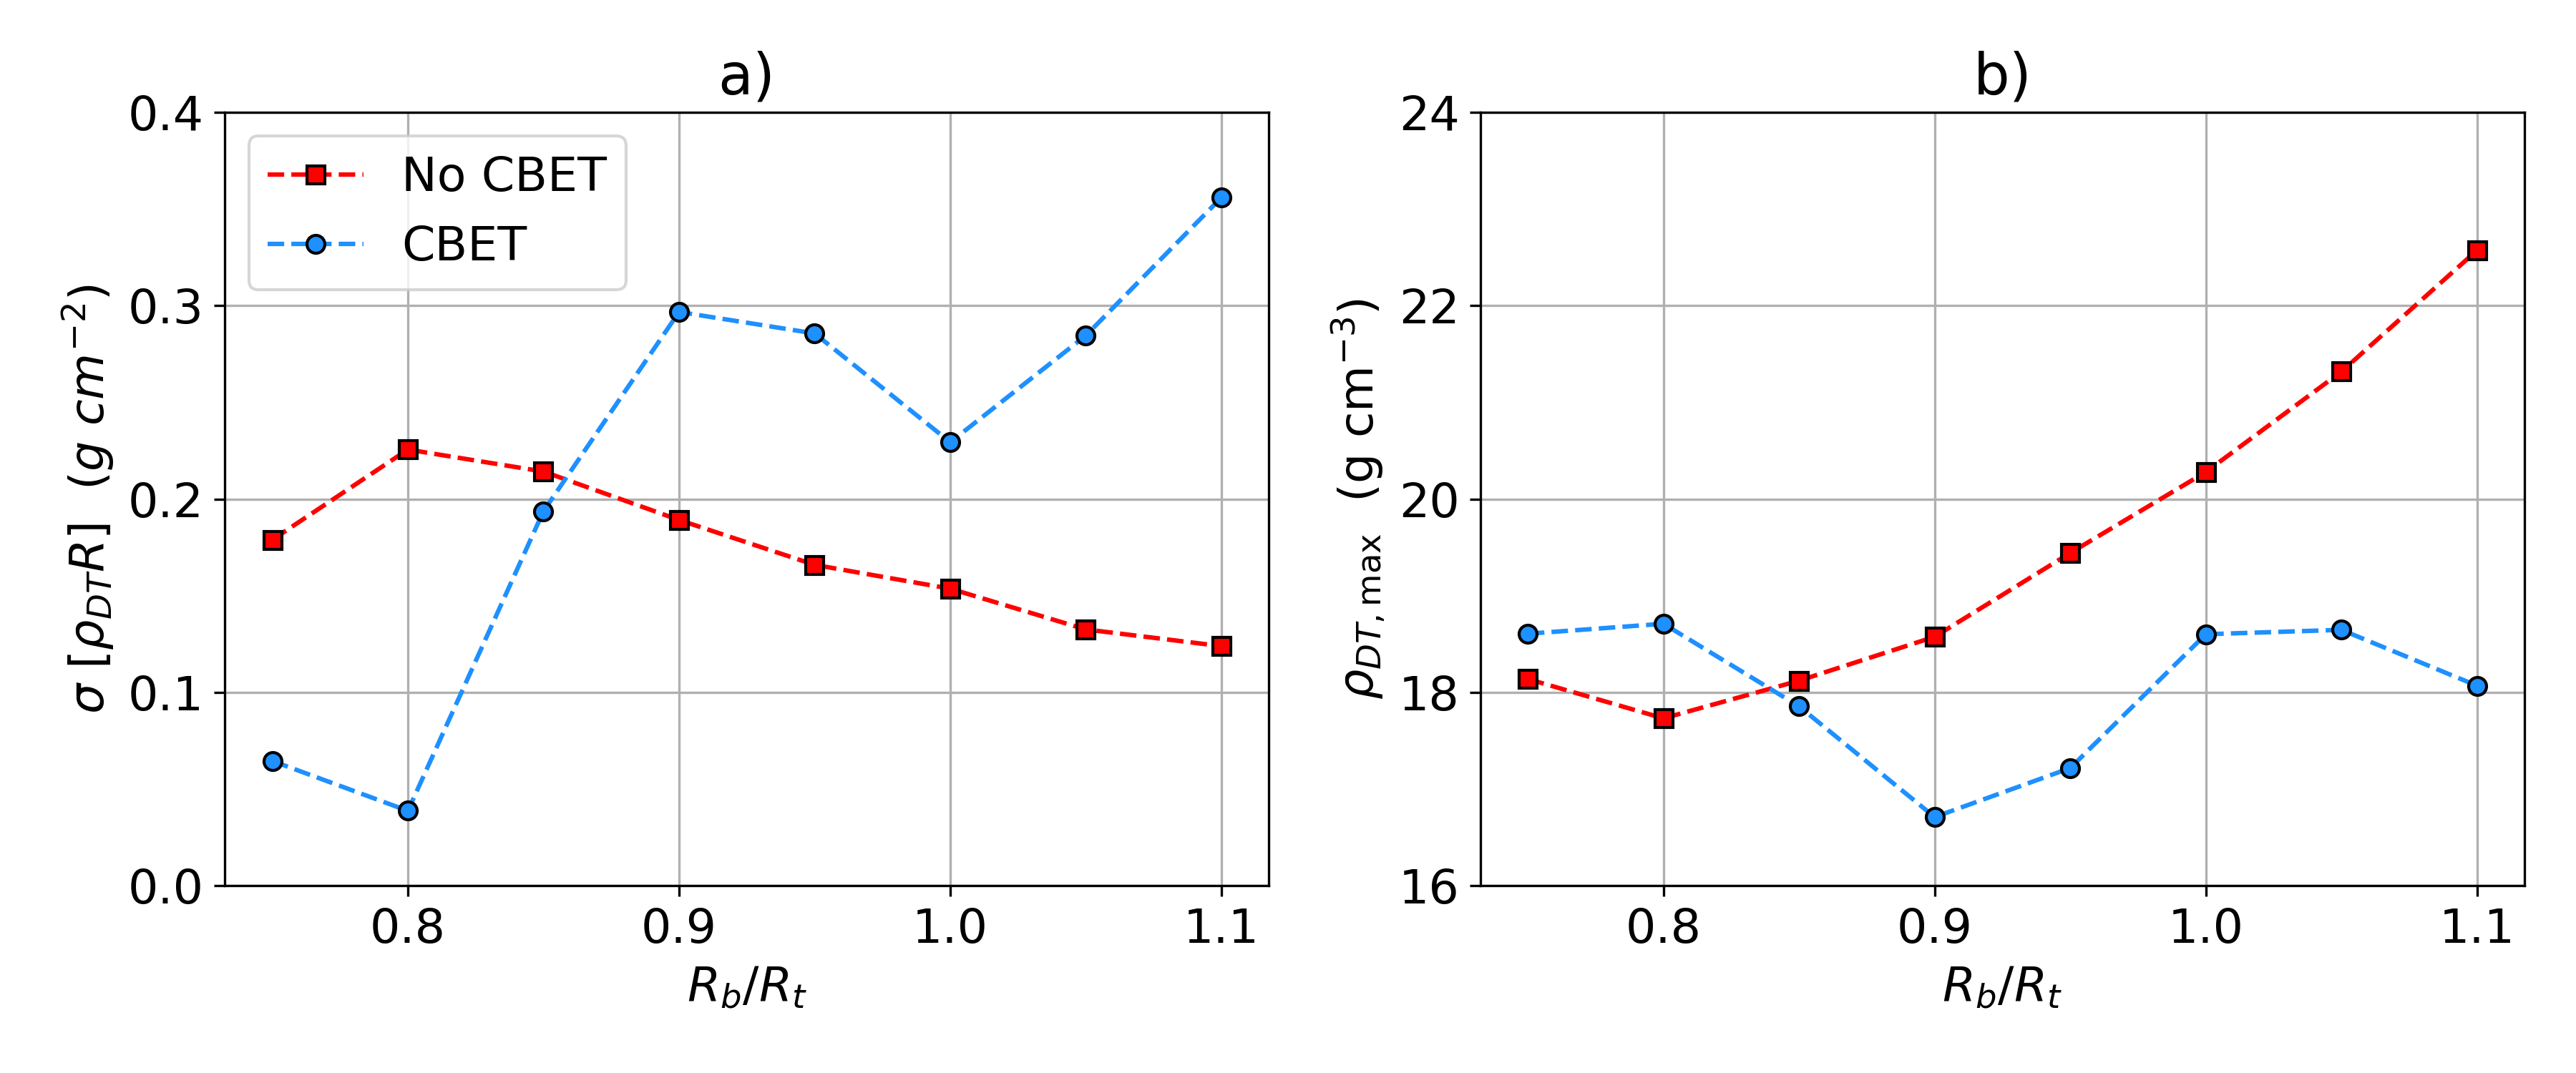
\includegraphics[width=1.0\linewidth]{Results1/Images/RbRt_sig_rhomax.png}
    \centering
    \caption{Trends of a) stagnation asymmetry and b) maximum (azimuthally averaged) fuel density for \ac{CBET} and no \ac{CBET} simulations.
    The no \ac{CBET} improvement in symmetry with $R_b/R_t$ is observed which also corresponds to improved compression.
    The symmetry trend including \ac{CBET} is more complex, but broadly the stagnation state symmetry is worse with increasing $R_b/R_t$.}%
    \label{fig:Res1_asymm_trend}
\end{figure}


%################################################################################
%################################################################################
\subsection{Time Resolved Asymmetry Growth}%
\label{sec:Res1_time_res_growth}

\begin{figure}[t!]
    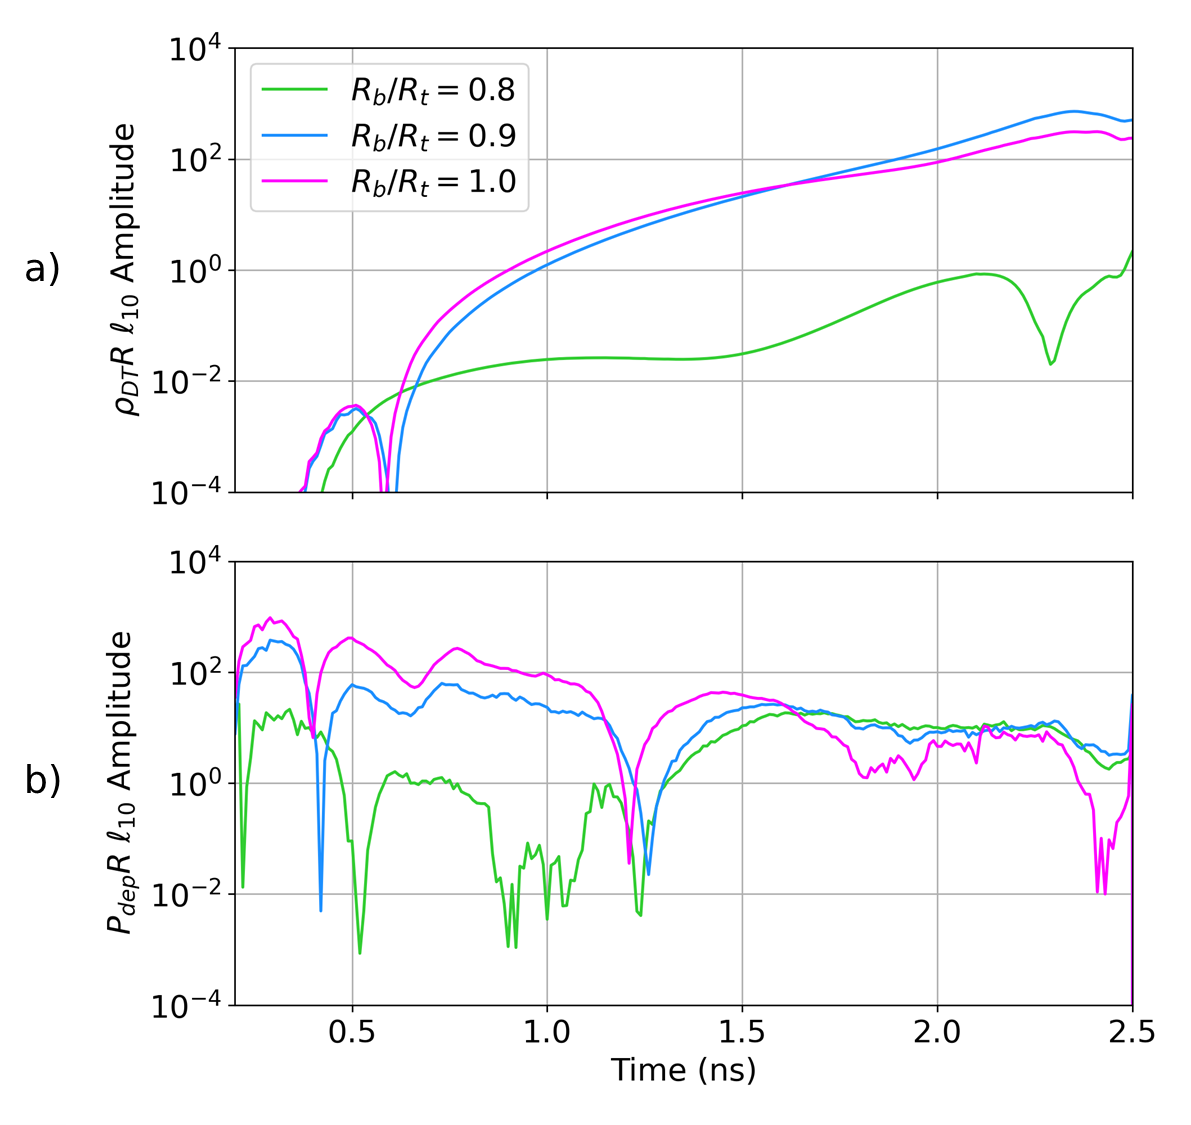
\includegraphics[width=0.75\linewidth]{Results1/Images/RbRts_mode10_growth.png}
    \centering
    \caption{Time resolved $\ell=10$ Fourier power spectrum amplitude for a) $\rho_{\text{DT}}R$ and b) $P_{\text{dep}}R$ for \ac{CBET} simulations with 3 $R_b/R_t$ values.
    The developing but unrealised modal flip for $R_b/R_t=0.8$ from $t \sim 0.5\rightarrow 1.2\ \text{ns}$ reduces the $P_{\text{dep}}R_{\ell=10}$ leading to slow $\rho_{\text{DT}}R_{\ell=10}$ growth and ultimately a relatively symmetric stagnation state.
    %Note that this developing but unrealised modal flip is clearly visible from reduced $P_{\text{dep}}R$ asymmetry values in Fig.~\ref{fig:Res1_PR_CBET_modes}.a.
    Despite large values of $\rho_{\text{DT}}R_{\ell=10}$ initially, the developing modal flip of the $R_b/R_t=1.0$ simulation from $t \sim 1.8\rightarrow 2.1\ \text{ns}$ slows the density asymmetry growth.}%
    \label{fig:Res1_mode10_growths}
\end{figure}


%###############################################################################################################################
%###############################################################################################################################
%###############################################################################################################################
\section{Conclusions}%
\label{sec:Res1_Conclusions}


%################################################################################
%################################################################################
\subsection{Summary of work}%
\label{sec:Res1_Summary}


%################################################################################
%################################################################################
\subsection{Future Work}%
\label{sec:Res1_future}